%
\documentclass[10]{article}
\usepackage{graphicx}
\begin{document}
\title{Step 2 - Work Log \\
M2M Lectures\\
Grenoble University}
\author{Stephane BERGER- Jean-Yves Bottraud}
\date{\today}
\maketitle

\section{Preface by Pr. Olivier Gruber}

This document is your work log for the second step in the 
M2M course, leading to build your own mini-distribution.

Like for the first step, this work log has two parts. 
One part is about diverse sections, that you must fill up.
Each section has a bunch of questions to help you do that.
The questions provide a guideline for your learning. 
They are about giving your pointers on what to learn about.
The other part is really a laboratory log, 
keeping track of what you do, as you do.

{\bf REMEMBER:} plaggia is a crime that can get you evicted
forever from french universities... The solution is simple,
write using your own words or quote, giving the source of
the quoted text. Also, remember that you do not learn through
cut\&paste. You also do not learn much by watching somebody else
doing.

\section{Outline of Step2}

To build your own distribution, almost from scratch, you will need
to acquire a number of skills:

\begin{itemize}
\item
GRUB bootloader
\item
Linux kernel
\item
Distribution layout and core files
\end{itemize}

Many pieces are provided to you, pieces that you are asked to understand.
First, you are given a compiled, ready-to-use, boot loader (GRUB 0.97).
Second, you are given a minimal distribution, with a linux kernel.

You can build a Qemu disk with mkdist.sh sript, following the on-screen
instructions. Once you have a disk, you can boot Qemu with it.
When booting, you will get a GRUB menu, with several boot options,
one is called ``Hello - RootFS''.
Select that option and you will get something very similar 
to what you did in step1, but using a real bootloader and a linux kernel.

After that, the learning process will start and it cannot be done entirely 
as a linear process, sorry. So you will fill up the various sections
incrementally, certainly in an order that will be a bit erratic.

We suggest the following steps.

\begin{enumerate}
\item Bootable disk and GRUB
\begin{itemize}
\item Read and start understanding the script: mkdist.sh
Explain each step, explaining the related concepts such as 
the loopback mount, mknod files (character and block).\\

\textbf{loopback }: pouvoir travailler sur un disque dur sur notre syst\`eme alors que le disque n'existe pas physiquement. On va cr\'eer un fichier (de type block ou charater )rempli de 0 d'une certaine taille . Apr\`es on va lier ce fichier \`a un loop device libre(8 loop device disponible sous linux).
Ensuite on peut le formater (mkfs) et le monter (mount).
on effectue une simulation d'un disque dur, d'un cd , d'un mat\'eriel.

\textbf{Block device }: (fichier sp\'ecial de type bloc) C'est un device file dans lequel le syst\`eme transf\'erera les donn\'ees sous forme de blocs.
On a la possibilit\'e de faire un acc\`es non sequentiel au xdonn\'ees (buffering,acc\`es al\'eatoire) C'est le cas du disque dur.\\

\textbf{Charactere device :} 
Fichier sp\'ecial de type caract\`ere =
 C'est un device file dans lequel les donn\'ees seront transmises caract\`ere par caract\`ere (sequntiel). exemple : port s\'erie\\

pour voir les devices dans Unbuntu : ls -l /dev\\
\textbf{b = block device}\\
brw-rw----  1 root    disk      7,   0 fevr.  8 09:29 loop0\\
brw-rw----  1 root    disk      1,   0 fevr.  8 09:29 ram0\\ 
brw-rw----+ 1 root    cdrom    11,   0 fevr.  8 09:29 sr0\\\\
rm: sr0 est de type block, c'est le cd des additons pour virtualbox

\textbf{c = charactere device}\\
crw--w----  1 root    tty       4,   0 fevr.  8 09:29 tty0

\item Read about and understand the GRUB process and how it is installed on a disk and the GRUB boot stages.

Sur le disque il faut sur le MBR le stage 1 ()
ensuite on  place le Stage 1.5 pour que certains driver sp\'ecifique soit charg\'es si n\'ecessaire.  ( dans les 30 kilooctets suivant le MBR).
Stage 1 charge Stage 1.5 si il est pr\'esent sinon il charge Stage 2.La partie 1.5 peut contenir des pilotes pour pouvoir acc\'eder \`a la partie 2.
Stage 1.5 charge  Stage 2 qui est plac\'e sur . 


\item Read about and understand the GRUB menu given to you.\\




\end{itemize}

\item Hello - RootFS
\begin{itemize}
\item Understand the first boot option of the GRUB menu (Hello - RootFS).
Which kernel boots? \\
vmlinufz-2.6.31-22-generic (cf menu.lst dans minidist/boot/grub)\\
What is the role of initrd.hello? \\
le r\^ole d'initrd est de permettre au chargeur d'amor\c cage de monter un disque RAM (system de fichier) \`a partir duquel il est possible de lancer des ex\'ecutables (le hello int\'egr\'e \`a initrd)et ensuite charger un autre syst\`eme de fichier\\

Look at the hello directory and how hello is compiled, linked, and the initrd.hello is constructed. 
Explain how it works and why.\\

le fichier initrd est le r\'esultat de la commpression de l'ex\'ecutable hello par cpio .
Hello a \'et\'e compile avec l'ensemble des biblioth\`eques n\'ecessaires \`a son  fonctionnement \\
dans le format ‘newc’ :
    The new (SVR4) portable format, which supports file systems having more than 65536 i-nodes. (4294967295 bytes).
    
Donc initrd.hello est une archive qui sera d\'ecompr\'ess\'ee puis ex\'ecut\'e apr\`es avoir \'et\'e charg\'ee en ram\\


\item Read about and understand the purpose of initial ramdisks (initrd)
for booting linux in general, on any machine.
\end{itemize}

\item Hello - Disk
\begin{itemize}
\item Read and understand the second boot option (Hello - Disk).
What is different in the boot process? \\
la diff\'erence est \\
	- le noyau qui n'est pas le m\^eme\\
	- le systeme de fichier est maintenant stock\'e sur hda1. le systeme boot alors sur /hello\\
Explain how this process boots the linux kernel from the disk you created with mkdist.sh.\\
le process va rechercher le noyau dans le r\'epertoire /boot/vmlinuz 
qui se trouve sur le systeme de fichier /dev/hda1 et puis ensuite il va  lancer l'intialisation avec l'executable hello qui se trouve \`a la racine du systeme de fichier.\\
\item Explain the two console options given to the kernel?\\
L'os va utiliser \\
	- le port s\'erie (ttyS0 = First UART serial port), 115200 bauds, pas de parit\'e sur 8 bits\\
	- une console vituellle (tty0 = Current virtual console)
Why are they useful?
ils vont permettre de 
 How do you exploit them when booting from Qemu?
\item Why do we use a different kernel for this boot process?
???????????????????
Instead of using the generic vmlinuz-2.6.31-22???????????????????
\item Compare the different kernel configurations given to you:
allnoconfig-2.6.32.65, miniconfig-2.6.32.65, m2m-config-2.6.32.65.
(hint: compiling a linux kernel, make allnoconfig, make bzImage)
(hint2: look at Section~\ref{sec:linux:kernel:config})

\end{itemize}

\item MiniDist Layout
\begin{itemize}
\item Dive into the given MiniDist and explain its layout,
giving the purpose of the different directories.
/boot : r\'epertoire contenant les noyau qui seront utilis\'es au boot
/boot/grub : les 3 stages de grub, un fichier de mappage pour le cd ou le disque et un fichier pour le menu. 
---> quelle diff\'erence entre boot et initrd ? ??????????

\item Explain the purpose of the few files in those directories.
In particular the various files under /dev.
dans /dev contient les differents devices (r\'ef\'erence au driver indentifie par un couple de chiffre mineur, majeur) qui peuvent être mont\'es.

\item What is missing for a realistic minidist?
tout 
(hint: libraries, commands, shell, configuration files and scripts).
\end{itemize}

\end{enumerate}

Here are a bunch of questions and points to help you progress
and focus your attention.

\begin{enumerate}
\item
Layout of the Qemu disk, in terms of GRUB stages and file system partition.
\item
Partition table in the MBR (see parted and fdisk)
\item 
What kind of file system are we using. ext2
Why only ext2? Could we use something other format? ext4
What do we have to pay attention to? Think GRUB
and Linux kernel. il faut que le SF sooit compatible Grub et linux
\item
Look in the GRUB manual how to install GRUB manually.
Explain the manual steps during the mkdist.sh.

Explain why they are necessary. 
dans le mbr il n'y a pas assez de place pour un vrai noyau , on y place alors juste un petit code (Stage 1) qui va charger le satge 1.5 ou le stage 2.

les deux autres stages sont  plus cons\'equants. Stage 1.5 sert \`a charger certains driver puis Stage 2

Stage2 sert a installer les derniers driver et \`a charger le Sf du systeme d'exploitation
\item
Explain the loop-back setup with the Qemu disk.
le disque est un fichier, il est donc virtuel. 
Why is it necessary? 
\item 
What are those files under /dev?
What is their purpose? How are they created? (hint mkdnod)
il ssont cr\'e\'es avec mknod en d\'efinissant le nom et les num\'ero mineur et majeur. Ces deuc num\'ero sontles identifiants pour les drivers mat\'eriels (norme) il ne sont pas d\'efinit comme ça, il ont une signification pr\'ecise 
voir : http://www.lanana.org/docs/device-list/devices-2.6+.txt
\item 
During the mkdist.sh, we boot Qemu twice in a row, 
with a manual GRUB setup in between.
What is going on? 
dans un premier temps on charge le console Grub et on lui donne le root et ensuite l'installe sur le disque (root) 
Explain why we stop at the GRUB prompt the first time
and why we get a GRUB menu the second time around.
la seconde fois on a un menu qui permet de choisir quel OS (noyau) booter.
\item 
Look at the GRUB menu and understand its structure.
titre afficher
le noyau et le fs
le boot
\item 
Look at the linux kernel options in the GRUB menu.
What are they for? Why use those options?

Hint: console history, see the differences between
booting Hello-RootFS and Hello-Disk.
\item
In your mini distribution, under /boot, you have
several kernels. Regarding the 2.6.31.22-generic,
what are the different files related to this version
(System.map, config, and vmlinuz).
\item
Explain how the linux kernel boots with Hello-RootFS.
Hint: initial ramdisk (initrd).
\item
Explain how the hello program can actually execute?
Indeed, the mini distribution has no libraries.
Hint: hello makefile.
\item 
Try replacing the kernel in the Hello-Disk configuration,
from vmlinuz to vmlinuz-2.6.31-22-generic, what is happening?
Why? Why is it working with vmlinuz.
vmlinuz contient les drivers pour les disques durs (hda) mais pas vmlinuz qui est plus l\'eger (utilise la ram).


\end{enumerate}



\section{Qemu}

This section is here in case you learn some more stuff about Qemu.
You will find plenty of information in the README-QEMU document.

\section{MiniDist Script}

You ask to read and explain the following script (mkdist.sh).
\subsection{script mkdist.sh explanation }
\begin{enumerate}
\item 
compilation de l'executale hello et int\'egration dans une archive d'un systeme de fichier racine (root file systeme) = distribution
\item 
Cr\'eation du fichier disque (fichier minidist.img) (secteur de 512 octets)
	1 secteur : fichier stage 1
	secteur 2 \`a 198 : fichier stage 2 
	64 Mo de vide
\item Cr\'eation de la partition EXT2

\item Montage de la partition
\item Copie de la distribution (archive) sur la partition mont\'ee
\item synchronisation (sync - flush file system buffers)
\item D\'emontage de la partition
\item lancement de minidist.img avec Qemu pour installation et configuration de GRUB (Bootloader)
\begin{itemize}
\item \textbf{grub : root (hd0,0)}\\
\textit{commande} : <device-type><device-number>,<partition> \\
\textit{definiton} :   Configure la partition root de GRUB et monte la partition.
\item \textbf{grub : setup (hd0)} \\
\textit{definition} : cette commande installe GRUB sur le MBR du premier disque (hd0).
\item \textbf{grub : halt}\\
\textit{definiton} : quitter 
\end{itemize}
\item lancement de minidist.img avec Qemu pour lancer le systeme install\'e et donc le fichier ex\'ecutable Hello

\end{enumerate}

\section{GRUB} 

In the grub directory, you will have binary and the sources for
grub-0.97, an older and much simpler GRUB version.
\\sources infos :\\
$http://www.linux-france.org/article/sys/chargeurs/ix86/grub/grub-manual-fr.html\#fn-1\\
http://lea-linux.org/documentations/Grub\\
https://www-uxsup.csx.cam.ac.uk/pub/doc/suse/suse9.2/suselinux-adminguide_en/ch07s04.html\\
https://docs.oracle.com/cd/E37670_01/E41138/html/ch04s02.html$

\subsection{Qu'est-ce que GRUB ?}
\subsubsection{Pr\'esentation}
GRUB (ou GNU)est un chargeur de d\'emarrage \`a  l'instar de LILO. Il est extr\^emement flexible et peut charger un syst\`eme sans enregistrer la position physique du noyau sur le disque. Vous pouvez lancer un noyau simplement en pr\'ecisant son nom de fichier et le disque (et la partition) sur lequel il r\'eside. Pour ce faire, vous pouvez utiliser l'interface ligne de commande ou l'interface menu. Il est inutile de relancer GRUB apr\`es une modification de sa configuration. Toute modification du fichier de configuration /boot/grub/menu.lst est imm\'ediatement prise en compte. Rappelons enfin que Linux peut être install\'e sur n'importe quelle partition. 
GRUB utilise la technique standard pour charger un OS ou du chargement chaîn\'e (chain-loading), pourcharger des syst\`emes d'exploitation non-support\'es en activant un autre chargeur.
\subsubsection{Principe}
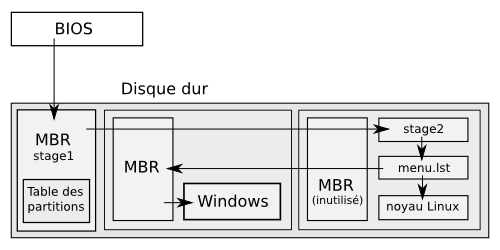
\includegraphics{SchemaSimplifieGrubDualBoot}
\textit{Sch\'ema simplifi\'e d'un dual-boot}
\subsubsection{rappels}
\textbf{(hd0,1)}\\
Ici, hd signifie qu'il s'agit d'un disque dur. Le premier nombre 0 indique le num\'ero du disque, qui est ici le premier disque, alors que le second entier 1 indique le num\'ero de la partition (ou le num\'ero de slice dans la terminologie BSD). Encore une fois, notez que les num\'eros de partitions sont d\'etermin\'es \`a partir de z\'ero, et non depuis un. Cette expression d\'esigne la deuxi\`eme partition du premier disque dur. Dans ce cas, GRUB n'utilise qu'une partition du disque \`a la place du disque entier.  

\textbf{root device} [hdbias] 	

D\'efinit le device comme \'etant la partition racine, puis essaie de la monter pour obtenir la taille de la partition (pour passer le descripteur de la partition en ES:ESI, utilis\'e par certains chargeurs chaîn\'es), le type de disque BSD (pour d\'emarrer des noyaux BSD en utilisant leur format de d\'emarrage natif), et d\'eterminer correctement la partition PC ou se trouve la sous-partition BSD. Le param\`etre facultatif hdbias est un nombre pour informer un noyau BSD du nombre de disque BIOS qui se trouvent sur un contrôleur avant le disque actuel. Par exemple, s'il y a un disque IDE et un disque SCSI, et que votre partition racine FreeBSD se trouve sur le disque SCSI, utilisez 1 pour hdbias. 

\subsection{GRUB principles and stages}


\begin{enumerate}
\item
Look at eltorito stage for CD-ROMs. 

\begin{enumerate}
source : https://fr.wikipedia.org/wiki/El\_Torito
\item R\^ole\\ 
El Torito (de son nom anglais complet El Torito Bootable CD Specification) est une extension \`a la norme ISO 9660 sur les CD-ROM d\'ecrivant comment un ordinateur peut d\'emarrer - ou "booter" - \`a partir d'un CD-ROM
\item Fonctionnement\\
Selon la norme El Torito, le BIOS d'un PC r\'ecent peut rechercher un programme de boot sur un CD compatible ISO 9660. Si c'est le cas, le BIOS va alors assigner un num\'ero de p\'eriph\'erique au lecteur de CD. Ce num\'ero sera soit 80 (\'emulation du disque dur), 00 (\'emulation du lecteur de disquettes) ou un num\'ero au hasard si aucune \'emulation n'est n\'ecessaire.

Les \'emulations sont principalement utilis\'ees pour permettre \`a d'anciennes version d'OS de d\'emarrer \`a partir d'un CD en leur faisant croire qu'il d\'emarrent \`a partir d'un disque dur ou d'un lecteur de disquette.
\end{enumerate}

\item
Look at the various stages for a disk (stage1, stage1.5, stage2).
\begin{enumerate}
\item stage 1\\
Le premier niveau de GRUB se situe dans le MBR. Comme ce premier niveau ne peut \^etre que tr\`es petit puisqu'il n'y a que peu de place \`a disposition dans l'enregistrement d'amor\c cage maître ou dans les secteurs d'amor\c cage, la seule tâche de ce niveau est de charger le deuxi\`eme niveau de GRUB.soit le stage 1.5 ou directement le 2.
\\
pour le code : /boot/grub/stage1

\item stage 1.5\\
La partie 1.5 peut contenir des pilotes pour pouvoir acc\'eder \`a la partie 2
\item stage 2\\
Le deuxi\`eme niveau de GRUB fournit les fonctions r\'eelles du chargeur d'amor\c cage : entre autres le menu de choix (ou cache l'interpr\'eteur de commandes) et le code du programme avec lequel le contr\^ole de l'ordinateur est pass\'e au syst\`eme d'exploitation.. Lors de l'installation du chargeur d'amor\c cage, l'emplacement physique du disque dur dans lequel se trouve le second niveau est signal\'e dans le fichier du premier niveau.
\\
pour le code :  /boot/grub/stage2
\\
You can find some relevant documentations in the docs directory,
in particular the GRUB manual and a great explaination of QEMU disk
images.

\end{enumerate}
\item
Look in the GRUB manual how to install GRUB manually.
\item 
Look at GRUB menu.
\end{enumerate}

\subsubsection{Building GRUB}

{\bf --- THIS SECTION IS FOR YOUR INFORMATION ONLY --- },

{\bf Do not rebuild GRUB}, unless you have to and you are damn sure. 
You have been given a working for x86\_32 (IA-32). 

For your information, be warned that to build this version of GRUB, 
you will need GCC-3.4. So you can install it on your system, via apt-get install.
Let's assume you have downloaded your sources under ~/M2M/grub/grub-0.97
in your dev guest. You can compile and install like this:

{\em\small
\begin{verbatim}
        # export CC=gcc-3.4
	# cd ~/M2M/grub/grub-0.97
	# ./configure –prefix=~/M2M/grub/grub
	# make
	# make install 
\end{verbatim}
}

Notice the important setup in the configure step
where you specify a path where to install GRUB.
Notice this is a local path to your home directory,
{\bf DO NOT INSTALL IT ON YOUR MACHINE.}
By default, it installs on /boot/grub
and this is a really bad idea.

\section{GRUB and Linux Boot Process}

Look at what is going on in the /boot directory.
The idea here is to be able to explain the boot process,
starting with GRUB and ending with the linux kernel booting.

You must understand the three options in the GRUB menu.

\begin{enumerate}
\item
Hello - RootFS
\item
Hello - Disk
\item
Your Mini Distribution
\end{enumerate}

Each represents a different boot strategy.

\section{Linux Kernel Configurations}
\label{sec:linux:kernel:config}

You are given three configurations:

\begin{enumerate}
\item allnoconfig-2.6.32.65
\item miniconfig-2.6.32.65
\item m2m-config-2.6.32.65.
\end{enumerate}

All three for the version 2.6.32.65 of the linux kernel.

The all-no-config is generated with the ``make allnoconfig''
from a kernel source directory. It corresponds to the absolutely
smallest linux kernel, with all optional code turned off,
but it is no longer functional.

The mini-config is a functional kernel, corresponding to the
kernel given in the MiniDist, called vmlinuz. You are asked
to compare and explain the differences between the all-no-config
and the mini-config. 

\noindent (hint: a usefull program for this is called meld.)

\noindent (hint: the differences are related to the minimal
hardware support, like adding a pci bus support).

Then you are asked to do the same between the mini-config
and the m2m-config. The m2m-config is intended for a kernel
specifically compiled for our target distribution: small,
booting directly from disk, and with network connectivity.

You are asked the Qemu configuration that would correspond
to booting this kernel. (hint: look at README-QEMU).


\section{Mini-Distribution}

You are given this layout for your mini-distribution.
{\em\small 
\begin{verbatim}
  MiniDist> ls
  bin  boot  dev  etc  hello  lib  root  sbin
  MiniDist>
\end{verbatim}
}

Explain each directory and each directory's contents.

If you add anything, you will document what you add and why.

\section{Laboratory Log}
 \subsection{Initrd}
 voir $http://artisan.karma-lab.net/customiser-initrd$

\end{document}
